\chapter{Results}	

This analysis focused on a sample of 6,364 rural census tracts with a RUCA code of seven or higher. Four states and Washington D.C. were intentionally excluded from the analysis: Alaska and Hawaii were omitted due to the presence of unique factors, particularly in their rural areas, which may not have been adequately addressed in the existing literature.  New Jersey and Rhode Island were excluded from our spatial analysis due to a lack of adequate data. These states are both very urban and once discrepancies in the data were removed, there were not enough observations to include in the analysis.  Figure \ref{fig:neighbors_bar} shows how the neighbor algorithm changed the state census tract counts. 

\begin{figure}[htbp]
    \centering
    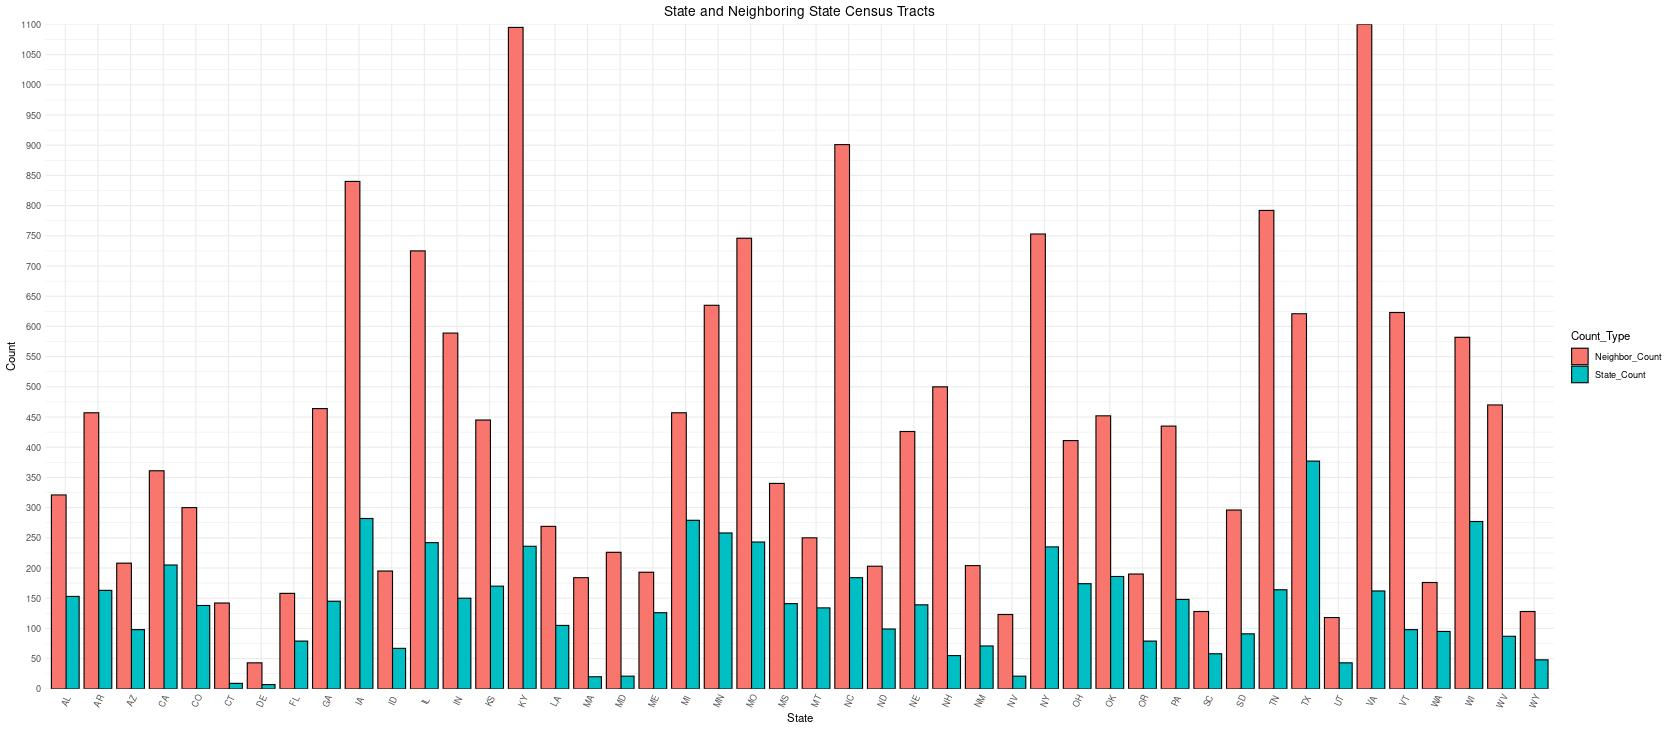
\includegraphics[width=1\textwidth, height=10cm]{plots/neighbors.jpeg}
    \caption{State Census Tracts vs. State Neighbors Count}
    \label{fig:neighbors_bar}
\end{figure}


\section{\textit{Cluster Analysis}}

Here, the results of the cluster analysis is presented for each sector. The primary mechanism for analyzing the clusters is the average cluster medians for all states. The cluster averages were analyzed as well to ensure that the same trends are found in the dataset under a different descriptive statistic. All values are represented as a percentage corresponding to the base unit each sector is scaled to. 

\subsection{\textit{Employment Diversity}}
The risk levels for employment diversity are determined based on which clusters have the highest number of highest cluster values compared to the cluster with the lowest number of lowest cluster values. The higher the cluster averages across variables, the better the economic diversity of a cluster. Table \ref{tab:emp} shows the values for this sector. 
Cluster 1 had the lowest cluster medians in 61 percent of variables, 
Cluster 2 has the highest cluster median in 53 percent of variables, and Cluster 3 has the middle value in 69 %nice 
percent of cases. Based on this analysis Cluster one has the lowest level of economic diversity, cluster two has the lowest level of economic diversity, and cluster three has a medium level of economic diversity. Employment in education, health, and social work has the highest presence across each cluster followed by manufacturing. 

% latex table generated in R 4.1.2 by xtable 1.8-6 package
% Thu Nov 23 19:11:59 2023
\begin{table}[ht]
    \centering
    \caption{Median Values for Employment Diversity Clusters}
    \label{tab:emp}
    \begin{tabular}{|r| r| r| r|}
        \hline
        Variable & Cluster 1 & Cluster 2 & Cluster 3 \\ 
        \hline
        ag\_for\_fish\_hunt\_mining & 2.54 & 2.24 & 1.87 \\ 
        \hline
        arts\_rec\_food & 2.86 & 3.12 & 3.10 \\ 
        \hline
        construction & 3.16 & 3.06 & 3.07 \\ 
        \hline
        edu\_health\_social & 9.38 & 9.73 & 9.46 \\ 
        \hline
        fin\_re\_insur & 1.47 & 1.60 & 1.57 \\ 
        \hline
        information & 0.35 & 0.41 & 0.37 \\ 
        \hline
        manufacturing & 4.52 & 5.44 & 4.75 \\ 
        \hline
        othersvcs & 1.76 & 1.88 & 1.91 \\ 
        \hline
        prof\_sci\_mgmt\_waste & 2.17 & 2.25 & 2.28 \\ 
        \hline
        public\_admin & 1.98 & 1.88 & 1.92 \\ 
        \hline
        retail\_trade & 4.48 & 4.78 & 4.59 \\ 
        \hline
        trans\_warehouse\_util & 2.17 & 2.03 & 2.12 \\ 
        \hline
        wholesale\_trade & 0.76 & 0.86 & 0.70 \\ 
        \hline
    \end{tabular}
\end{table}

\pagebreak

\subsection{\textit{Demographics}}

Due to the historical forces affecting minorities in both rural and urban areas, the risk levels for demographics are based on which clusters have the highest minority populations and the lowest white populations. 
Table \ref{tab:dem} shows the values for this sector.  This sector was decided based on the median and average highest, lowest, and medium value counts as clusters two and three had almost the same cluster median counts. Cluster three is the middle value for 90 percent of cluster median variables. Cluster three has the highest number of highest values across means and medians with 55 percent of variables. Cluster two is the lowest for 50 percent of variables. Cluster three alsos has the largest African American and Hispanic and Latino cluster medians. Based on this analysis, cluster one has a medium risk of housing insecurity, cluster two has a low risk of housing insecurity and cluster three has the highest risk of housing insecurity. One notable obeservation is that the cluster medians for the male/ female over 18 years old variables are roughly three times higher than the male/ female under 18 variables. This reflects the ageing population of rural areas noted in the literature. 

% latex table generated in R 4.1.2 by xtable 1.8-6 package
% Thu Nov 23 19:33:06 2023
\begin{table}[ht]
    \centering
    \caption{Median Values for Demographic Diversity Clusters}
    \label{tab:dem}
    \begin{tabular}{|r|r|r|r|}
      \hline
     Variable & Cluster 1 & Cluster 2 & Cluster 3 \\ 
      \hline
    am\_in\_ala\_nat & 0.21 & 0.28 & 0.18 \\ 
    \hline
      asian & 0.21 & 0.22 & 0.15 \\ 
      \hline
      black & 0.72 & 0.72 & 0.85 \\ 
      \hline
      female\_o18 & 39.25 & 40.15 & 38.90 \\ 
      \hline
      female\_u18 & 10.77 & 9.79 & 10.98 \\ 
      \hline
      haw\_pac & 0.00 & 0.00 & 0.00 \\ 
      \hline
      hisp\_lat & 2.92 & 2.63 & 3.08 \\ 
      \hline
      male\_o18 & 38.26 & 39.38 & 37.99 \\ 
      \hline
      male\_u18 & 11.44 & 10.27 & 11.70 \\ 
      \hline
      other & 0.32 & 0.30 & 0.41 \\ 
      \hline
      white & 94.35 & 93.67 & 92.52 \\ 
       \hline
    \end{tabular}
    \end{table}

\subsection{\textit{Housing Cost}}

For housing cost, risk levels are determined by which clusters have the highest cluster medians. Cluster 1 has the highest value for mortgage high cost. Cluster 2 has the lowewest mortgage and rent high cost cluster medians. cluster 3 has the highest no mortgage and rent high cost cluster medians. Table \ref{tab:cost} shows the values for this sector. Cluster one becomes the medium risk level, cluster two becomes the low risk level, and cluster three becomes the high risk level. 

% latex table generated in R 4.1.2 by xtable 1.8-6 package
% Fri Nov 24 09:55:27 2023
\begin{table}[ht]
    \centering
    \caption{Median Values for Housing Cost Clusters}
    \label{tab:cost}
    \begin{tabular}{|r|r|r|r|}
    \hline
    Variable & Cluster 1 & Cluster 2 & Cluster 3 \\ 
    \hline
    mortgage\_high\_cost & 5.22 & 4.35 & 4.93 \\ 
    \hline
      no\_mortgage\_high\_cost & 2.16 & 2.18 & 2.89 \\ 
    \hline
      rent\_high\_cost & 15.69 & 14.18 & 16.79 \\ 
    \hline
    \end{tabular}
    \end{table}

\subsection{\textit{Housing Quality}}

For housing quality, risk levels are determined by which clusters have the highest values, with preference given to occupied housing as housing conditions in unoccupied housing is of a lesser concern than occupied housing. Table \ref{tab:qual} shows the values for this sector. Cluster one has the highest values for unoccupied housing with incomplete kitchens and plumbing. Cluster three has the medium value for each variable.Cluster three has the highest values for occupied housing with incomplete kitchens and plumbing. Cluster one becomes the lowest risk level, cluster two becomes the medium risk level, and cluster three becomes the highest risk level. 

% latex table generated in R 4.1.2 by xtable 1.8-6 package
% Fri Nov 24 09:58:52 2023
\begin{table}[ht]
    \centering
    \caption{Median Values for Housing Quality Clusters}
    \label{tab:qual}
    \begin{tabular}{|r|r|r|r|}
      \hline
     Variable & Cluster 1 & Cluster 2 & Cluster3 \\ 
      \hline
    all\_incomplete\_kitchen & 25.85 & 25.76 & 19.75 \\ 
    \hline
      all\_incomplete\_plumb & 24.00 & 22.73 & 17.28 \\ 
    \hline
      occ\_incomplete\_kitchen & 0.46 & 0.52 & 0.64 \\ 
    \hline
      occ\_incomplete\_plumb & 0.00 & 0.11 & 0.34 \\ 
    \hline
    \end{tabular}
    \end{table}



\subsection{\textit{Residential Mobility: Education}}
For residential mobility: education, the risk levels are determined primarily by the variables for those who moved with less than a high school education and those in the same house with less than a high school education, and the clusters where more people moved overall will be the highest risk levels. Table \ref{tab:trans_edu} shows the values for this sector. Cluster one has the medium value for 71 percent of variables including each less than high school education variable. Cluster two has the lowest values for each variable. cluster 3 has the highest values for 71 percent of variables, including each of the less than high school education variables. Cluster one becomes the lowest risk level because it has medium levels of residential mobility but the highest level of residential stability with a high school education. Cluster two becomes the medium risk level, and cluster three becomes the highest risk level. 

% latex table generated in R 4.1.2 by xtable 1.8-6 package
% Fri Nov 24 10:02:45 2023
\begin{table}[ht]
    \centering
    \caption{Median Values for Residential Mobility: Education Clusters}
    \label{tab:trans_edu}
    \begin{tabular}{|r|r|r|r|}
      \hline
     Variable & Cluster 1 & Cluster 2 & Cluster 3 \\ 
      \hline
    moved\_diff\_county\_hs & 0.51 & 0.44 & 0.55 \\ 
    \hline
      moved\_diff\_county\_less\_than\_hs & 0.13 & 0.10 & 0.18 \\ 
      \hline
      moved\_diff\_state\_hs & 0.18 & 0.10 & 0.18 \\
      \hline 
      moved\_diff\_state\_less\_than\_hs & 0.00 & 0.00 & 0.00 \\
      \hline 
      moved\_in\_county\_hs & 0.95 & 0.84 & 1.36 \\ 
      \hline
      moved\_in\_county\_less\_than\_hs & 0.30 & 0.24 & 0.50 \\ 
      \hline
      same\_house\_hs & 23.99 & 22.60 & 22.97 \\ 
      \hline
      same\_house\_less\_than\_hs & 7.71 & 6.97 & 7.82 \\ 
       \hline
    \end{tabular}
    \end{table}

\pagebreak

\subsection{\textit{Residential Mobility: Poverty}}

The residential mobility: poverty sector follows the criteria of residential mobility: education closely with those the variables for those who moved that are below the poverty level are the highest priority. Table \ref{tab:trans_pov} shows the values for this sector. Cluster one has the lowest values for every variable. Cluster two has the medium value for 57 percent of variables. Cluster three has the highest values for 57 percent of variables including three of the below the poverty level variables. Cluster one becomes the lowest risk level, cluster two becomes the medium risk level, and cluster three becomes the highest risk level. One noteable observation from the cluster medians is that cluster three has the highest value of those living in the same house below and above the poverty measure, indicating high levels of poverty for \cts in this cluster.

% latex table generated in R 4.1.2 by xtable 1.8-6 package
% Fri Nov 24 10:09:00 2023
\begin{table}[ht]
    \centering
    \caption{Median Values for Residential Mobility: Poverty Clusters}
    \label{tab:trans_pov}
    \begin{tabular}{|r|r|r|r|}
      \hline
     & cluster\_1 & cluster\_2 & cluster\_3 \\ 
      \hline
    moved\_diff\_county\_p1 & 0.30 & 0.41 & 0.48 \\
    \hline 
      moved\_diff\_county\_p2 & 0.04 & 0.12 & 0.07 \\ 
      \hline
      moved\_diff\_state\_p1 & 0.05 & 0.10 & 0.08 \\ 
      \hline
      moved\_diff\_state\_p2 & 0.00 & 0.00 & 0.00 \\ 
      \hline
      moved\_in\_county\_p1 & 0.74 & 1.00 & 1.06 \\ 
      \hline
      moved\_in\_county\_p2 & 0.30 & 0.43 & 0.40 \\ 
      \hline
      same\_house\_p1 & 9.86 & 10.80 & 12.14 \\ 
      \hline
      same\_house\_p2 & 7.79 & 8.55 & 9.04 \\ 
       \hline
    \end{tabular}
    \end{table}

\subsection{\textit{Wage and Household Factors}}

For household wage/ aid, the clusters with the highest number of highest cluster medians determines the risk levels with particular attention given to households with no wage and households with three or more workers. Table \ref{tab:waid} shows the values for this sector. Cluster one has the lowest cluster medians for 89 percent of variables. Cluster two has the medium value for 55 percent of variables. Cluster three has the highest values for 55 percent of variables and the middle value for the other variables. Notablable high values for cluster three include the Gini indexx, households with no vehicle, households with at least one worker and no vehicle, and households receiving supplemental security income.  

% latex table generated in R 4.1.2 by xtable 1.8-6 package
% Fri Nov 24 10:25:00 2023
\begin{table}[ht]
    \centering
    \caption{Median Values for Household Factor Clusters}
    \label{tab:waid}
    \begin{tabular}{|r|r|r|r|}
      \hline
     & Cluster 1 & Cluster 2 & Cluster 3 \\ 
      \hline
    gini\_index & 42.69 & 42.91 & 44.07 \\ 
    \hline
      hh\_3plus\_worker & 1.85 & 1.67 & 1.81 \\ 
      \hline
      hh\_no\_investment\_income & 32.64 & 33.04 & 33.29 \\ 
      \hline
      hh\_no\_other\_income & 36.28 & 36.81 & 36.79 \\ 
      \hline
      hh\_no\_vehicle & 1.96 & 2.12 & 2.34 \\ 
      \hline
      hh\_no\_wage & 13.38 & 14.11 & 14.01 \\ 
      \hline
      hh\_public\_assistance & 4.84 & 5.54 & 5.40 \\ 
      \hline
      hh\_ssi & 2.17 & 2.39 & 2.51 \\ 
      \hline
      hh\_worker\_no\_vehicle & 1.28 & 1.45 & 1.59 \\ 
       \hline
    \end{tabular}
    \end{table}

\subsection{\textit{Housing Type}}

Table \ref{tab:hh_type} shows the values for this sector. 

% latex table generated in R 4.1.2 by xtable 1.8-6 package
% Fri Nov 24 10:28:27 2023
\begin{table}[ht]
    \centering
    \caption{Median Values for Housing Type Clusters}
    \label{tab:hh_type}
    \begin{tabular}{|r|r|r|r|}
      \hline
     Variable & Cluster 1 & Cluster 2 & Cluster 3 \\ 
      \hline
    owner\_2to4 & 0.00 & 0.00 & 0.00 \\ 
    \hline
      owner\_5plus & 0.00 & 0.00 & 0.00 \\ 
      \hline
      owner\_mobile & 8.29 & 10.06 & 10.41 \\ 
      \hline
      owner\_single & 90.75 & 88.67 & 88.42 \\ 
      \hline
      owner\_unconvent & 0.00 & 0.00 & 0.00 \\
      \hline 
      renter\_2to4 & 8.29 & 10.57 & 10.59 \\ 
      \hline
      renter\_5plus & 5.78 & 8.50 & 7.70 \\ 
      \hline
      renter\_mobile & 9.25 & 13.04 & 10.79 \\ 
      \hline
      renter\_single & 68.16 & 55.67 & 60.95 \\ 
      \hline
      renter\_unconvent & 0.00 & 0.00 & 0.00 \\ 
       \hline
    \end{tabular}
    \end{table}




\section{\textit{Association Rules}}
For 1:1 rules, the rule with the highest confidence and support is between housing type and cost, occurring in 11 percent of transactions with a coverage of 0.29. Wage/ household aid has the most one-one- associations in this group occurring in an average of 1 percent of observations, there is a 36 percent average probability that any of these sectors are in the consequent if wage/ household aid is in the antecedent. In about 9 percent of observations, residential mobility poverty is the consequent if mobility education is the antecedent with a 36 percent probability of a high risk for mobility poverty when there is a high risk of mobility education. mobility education also has an association with employment with 33 percent confidence and 8 percent support. 

Of the 3:1 rules with the top 10 highest confidence values, employment diversity has a relationship with every other sector. Support is low at 5 percent with an average confidence of 0.42 and a slightly positive average lift of 1.1. The two other highest rules are housing type to mobility poverty with support of around twelve percent and a confidence interval of 0.41 and employment to residential mobility poverty with support of six percent and a confidence interval of 0.4. Looking at the top ten 3:1 rules with the highest confidence values, the results are significantly different from the 3:1 rules Employment is in the consequent if any other sector is in the antecedent with an average support of 12 percent, and an average confidence interval of 0.32. This relationship between employment diversity having both high-risk-to-low-risk and high-risk-to-low-risk is a surprising relationship. 

\section{\textit{Moran's I}}

\textit{Figure 4 about here}

Moran’s I is calculated for every state and the entire dataset. With the exceptions of demographics and employment diversity, the average Moran's I statistics are between 0.2 and 0.35 (see figure 4). For demographics, African American has the strongest spatial autocorrelation at 0.49 followed by Whites at 0.45 and Hispanics and Latinos at 0.4. Jobs often considered more urban such as retail trade and information services have small positive spatial autocorrelations with values around 0.1. For household wage/ aid, the households with no wage variable have the highest average Moran’s I statistic at 0.34, followed by households with public assistance at 0.3. The most surprising observation in this sector is the Gini index. There is a lot of conversation in the public and academic spheres about income inequality, yet in rural areas there is an average Moran’s I of 0.19, indicating a very slight positive spatial autocorrelation. For housing cost, the most surprising observation is the low average spatial autocorrelation of high-cost renters. At only 0.16, there is not as much clustering of high rent burdened households in rural areas. mobile home ownership and single unit ownership have the highest spatial autocorrelations for housing type with Moran’s I values of 0.34.  Mobile home renters has an average Moran’s I of 0.22. Unconventional housing types for both owners and renters had slightly positive Moran’s I statistics at 0.2 and 0.15. For mobility education, same house without a high school diploma (0.34) and same house with a high school diploma (0.31) have similar values and while the positive spatial autocorrelations are low, they are notably higher than the mobility variables in the Sector. While same house below the poverty line had the strongest spatial autocorrelation of (0.27), moved different county at 125 percent of the poverty level (0.18) is between the two same house poverty level variables and almost identical to same house 125 percent of the poverty level when rounding to the third decimal place. For employment diversity, average Moran’s I statistics vary across all variables with manufacturing (0.47) and Black (0.49 having the highest values.  


\section{\textit{Multinomial Logistic Regression}}

The final method applied in this study is a multinomial logistic regression performed on each sector of data and tested on the data for each state. The probability that a predicted risk level is the actual risk level is used to measure how well the data for each state can be predicted based on a model trained on the other states. These probabilities are used to saturate the final map ) to visualize how well census tracts conform to the national dataset. Average accuracy for all sectors was low, ranging between 34  for employment diversity and 38 percent for demographics. Medians were in a similar range of 32 percent for mobility poverty and 40 percent for demographics. Demographics had the highest standard deviation at 14 percent, indicating a high degree of variation in predictability. Looking at average probability for each sector in each state, Utah had the best prediction results with an average of 41 percent and Minnesota was the hardest to predict at 31 percent between sectors. The standard deviation of every state is 14 percent, indicating a high level of variation in each state. While the standard deviation is significant, the mean and median statistics indicate the data is close to symmetrically distributed.  

\textit{Figure 5 about here}


\endinput